\chapter{Introduction} \label{chap:intro}
The goal of this thesis is the implementation of a parallel implementation of a pointer analysis. As well as researching to what extent such an implementation presents advantages or disadvantages over other analyses that are not strictly parallel in nature.

\section{Structure of this Thesis}
This thesis is divided into three chapters.
The first chapter \autoref{chap:intro} lays the groundwork for the implementation and goes into detail what ideas were persued in order to develop the implementation. All related current work and it's influences on this work is discussed here, as well as the motivation for the implementation itself. Furthermore the fundamentals of pointer analysis are explained here with code samples and an end to end analysis workflow that aims to illustrate the connection between actual code and its representation in a pointer analysis.

In the second chapter \autoref{chap:main} the software, namely PTAGPU, that was developed as part of this thesis, is described in detail. Design decisions, integrations with other software libraries and correctness are elaborated here.
The experimental benchmark results and how they wre generated are also presented here.

The last chapter \autoref{chap:conclusion} covers possible future work that could further improve the implementation and explore more ideas concerning parallel pointer analyses.
This chapter also discusses the experimental results from \autoref{chap:main}.


\section{Pointer Analysis}
In general a pointer analysis tries to find the values of pointers in a program at runtime, without having to execute the program.
So naturally this problem is undecidable \cite{landi1992undecidability} following a reduction from the halting problem.
As a result, pointer analyses have to produce an over-approximation of the targets each pointer can point towards at runtime.
One common pointer analysis is the inclusion-based Andersen Analysis \cite{andersen1994program}. The details of this type of analysis will be discussed later on, as it is the underlying basis for the proposed algorithm in \autoref{chap:main}. The Andersen algorithm sacrifices precision in favor of performance and achives an upper bound of $O(n^3)$ where n represents the program size. This is known as the cubic bottleneck of general Andersen Analysis \cite{mathiasen2021fine}.
This showcases the tradeoff that all non-theoretical pointer analyses have to make in oder to be applicable to real programs and avoid undecidability. Furthermore Andersen Analysis is a P-complete problem and is therefore not trivially parallelizable.

As a general abstraction, pointer analyses can be seen as complex graph problems where programs are interpreted as graphs with nodes representing variables and edges representing relations between nodes, such as memory allocations and assignments bewteen variables.
This allows us to make use of a large body of previous research concerning graph problems and transform the general analysis into a better defined mathematical problem.

Another analysis closely related to pointer analysis is alias analysis, where two pointers are said to alias if their points-to sets have an intersection. An alias analysis produces a set of relations over all nodes in the analysis graph where nodes can either \textbf{NotAlias}, \textbf{MayAlias} or \textbf{MustAlias}.
For two given nodes, $a$, $b$ and their points-to sets $pts(a)$ and $pts(b)$ the following constraints describe the relations.
$$a\ \textbf{NotAlias}\ b \iff \forall ptd \in pts(a) \colon ptd \notin pts(b)$$
$$a\ \textbf{MayAlias}\ b \iff \exists ptd \in pts(a) \colon ptd \in pts(b)$$
$$a\ \textbf{MustAlias}\ b \iff \forall ptd \in pts(a) \colon ptd \in pts(b)$$
Both pointer analysis, alias analysis, as well as points-to analysis are all terms commonly used interchangeably in literature \cite{hind2001pointer}. From now on pointer analysis will be used in this thesis to refer to this type of static analysis.

A motivating example for pointer analyses is the detection on memory leaks in programs.
This occurs when a memory location is allocated on the heap, for example with a call to malloc in glibc, and is not freed at a later stage in the program.
It is in the interest of the developer to find such faults as to not exhaust the computers memory during execution.
Finding such logical errors can be accomplished via a related static analysis called data-flow analysis, where each possible value at different stages of the program is calculated. Here pointer information is vital, as pointers can represent lateral movement of data trough the control flow of a program, independent of direct assignments and read operations. Ultimately almost all static analyses require some kind of information about pointers to fully determine the state of a program.
Aside from error detection such as memory leaks, optimizations are another aspect of compiler systems, where pointer information is important to achieve better results, see \autoref{lst:dataflow}.
More often than not the pointer information alone does not provide an immediate value to the compiler or analysis tool, instead other procedures build on top of this information to derive valuable information about a program.

\begin{listing}
    \begin{minted}{c}
    #include <stdlib.h>
    void *iter;
    iter = value;

    /* depending on the data at value's memory location 
    the loop might not be necessary */
    
    while(*iter)
    {
        complex_computation(iter);
    }
    \end{minted}
    \caption{Optimizations in a c program}
    \label{lst:dataflow}
\end{listing}

for example the liveness of a variable can be determined with pointer information. Since a given variable is considered live iff some following instruction

what is pta; survey \cite{hind2001pointer} and \cite{toman2017taming} and \cite{smaragdakis2015pointer}; theoretical complexity of parallel andersen analysis \cite{mathiasen2021fine}

\subsection{Notions of Sensitivity}
As previously established, a complete pointer analysis is undecidable.
For this reason there are various notions of sensitivity when talking about pointer analysis.
These notions present a compromise between precision and complexity of the analysis.
Following, some of the more common sensitivity notions will be illustrated to differentiate the more complex analyses from the less complex analyses and explain the impact of these sensitivities on actual performance when analyzing a program.

\subsubsection{Field-sensitivity}
\begin{minted}{c}
struct Person {
    char *name;
    int *age;
} p1, p2;
\end{minted}

Field-sensitivity describes how the pointer analysis algorithm handles structures in the program.
Most low-level languages, such as c, c++ and Rust, offer some form of structures to represent an object that internally holds multiple values.
If an analysis is field-sensitive, each field of each struct is represented in the analysis as an independent node that can point to unique memory locations.
For the given example, \verb|p1.age| and \verb|p1.name| can point to different memory locations.
Alternatively a field-insensitive analysis does not differentiate between any fields of a given struct.
Therefore only two nodes are created to represent the struct, $p1.*$ and $p2.*$.
Another common alternative is field-base-sensitivity, where instead of omitting the individual fields of each struct, the fields of every struct are merged into a single instance of that struct.
As a result the Person structs, p1 and p2, would be represented as a single object with fields name and age, such that \verb|p1.age == p2.age| are represented by the same node in the analysis.

\subsubsection{Array-sensitivity}
Array-sensitivity is conceptually similar to field-sensitivity but often has different effects on the runtime of the analysis.
For a given array $int arr[100]$ an array-sensitivie analysis would model each entry of the array, \newline e.g. arr[0], arr[1], \dots, with a unique node, whereas an insensitive analysis would model the array as a single node.
Generally speaking arrays are often homogeneous data structures that can hold a vast amount of data, compared to structs which are often more compact as they model attributes instead of raw data.
Therefore array-sensitivity if often omitted from whole program analyses, while field-sensitivity is common among pointer analyses.

\subsubsection{Scope of the analysis}
When designing a pointer analysis one has to make a decision about how to handle external code that the program depends on.
Often times a programs transitive dependencies can dwarf the original code by several magnitudes in size \cite{toman2017taming}.
Even a basic Hello World program in Java transitively depends on 3000 classes \cite{kulkarni2016accelerating} from the Java standard library.
For this reason most analyses either ignore external library code during analysis, or summarize the most relevant library calls during analysis, such as \verb|malloc| or \verb|free|.
Although this leaves most analyses in an unsound state, the tradeoff is well worth it, as most interesting properties in pointer analysis do not originate in standard libraries, but the actual program code that is written by the developer.
Furthermore, most standard libraries of common programming languages go through rigorous testing, making it exceedingly unlikely to produce errors.
This does however not solve the problem of standard library code mutating the program state. Here, simply ignoring the external code during analysis would greatly decrease the accuracy of the analysis.
For this reason, a lot of research is being done to develop methods that alleviate some of the problems that arise from analyzing external dependencies of a given program. Caching incremental results during analysis seems to be one of the most promising methods thus far \cite{mcpeak2013scalable}.

\subsubsection{Interprocedural analysis}
Another aspect that greatly influences the precision of analyses is whether they are interprocedural or intraprocedural.
An intraprocedural analysis only analyzes each function in an isolated context and disregards any influences on other functions or global state.
Interestingly most compilers rely mostly on intraprocedural analysis for bug detection as it can be performed in parallel for each function independently and is in general much faster than interprocedural analysis.
The following example \ref{lst:intraprocedural} illustrates the shortcomings of only performing intraprocedural analysis. Essentially parameter passing especially of pointers is not taken into account properly for the calculation of points-to sets.
An interprocedural analysis overcomes these limitations by connecting parameters of functions and the arguments at the respective callsites as well as the resulting return values in the graph structure that is used to solve the pointer analysis.
Fundamentally an interprocedural analysis is related to another notion of sensitivity, context sensitivity, since every context sensitive analysis has to be interprocedural in order to capture the context of each function call \cite{lin2015alias}.

\begin{listing}
    \begin{minted}{c}
        int *manupulatePointer(int *ptr);
        int main() {
            int *a, *b;
            b = manupulatePointer(a);
            /* intraprocedural analysis is unable 
            to determine the state of a or b */
        }
    \end{minted}
    \caption{Limitations of intraprocedural analysis}
    \label{lst:intraprocedural}
\end{listing}


\subsubsection{Flow-sensitivity}
When one performs a flow-sensitive pointer analysis, this means that instead of computing a single result for the entire program during analysis, 
one such result is computed during every possible step in the execution flow of the program.
As can be seen in \ref{lst:flowsens}, a flow-sensitive analysis is in general more precise than a flow-insensitive analysis. Meanwhile running a flow-sensitive analyis is also exponentially more expensive to compute as every step in a programs execution carries its own state concerning points-to relations - especially when the control flow is complicated by complex conditional statements or recursive execution.
Although this problem can be slightly alleviated, by only condering program statements that manipulate pointers.

\begin{listing}
    \begin{minted}{c}
        int *manupulatePointer(int *ptr);
        int main() {
            int a, b, *x; // x -> {}
            x = &a; // x -> {a}
            x = &b; // x -> {a,b} ?
            manupulatePointer(x);
            /* a flow insensitive analysis computes 
            a points-to set {a,b} for x while in actuality 
            x = &b overwrites x = &a during execution */
        }
    \end{minted}
    \caption{Flow-sensitivity by example}
    \label{lst:flowsens}
\end{listing}

\subsubsection{Context-sensitivity}
As previouly eluded to, context-sensitivity is directly related to interprocedural analyses, since it governs how call sites and called functions are interpreted in the analysis.
More specifically a centext-sensitive analysis considers the relevant program state at every function call, for this reason context-sensitive analyses are also flow-sensitive.
While a context-sensitive analysis would in theory provide more precision and therefore decrease the average size of points-to sets, in practice most context-sensitive analyses quickly grow out of control as the analysis explodes in terms of running time and space requirements \cite{smaragdakis2014introspective}. In contrast, context-insensitive analyses scale uniformly well.

\begin{listing}
    \begin{minted}{c}
        int *manupulatePointer(int *ptr);
        int main() {
            int a, b, *x;
            x = &a;
            manupulatePointer(x);
            x = &b;
            manupulatePointer(x);
            /* a context-sensitive analysis evaluates both
            calls to manupulatePointer as unique function calls
            since the context differs between both calls */
        }
    \end{minted}
    \caption{Context-sensitivity by example}
    \label{lst:contextsens}
\end{listing}

heap abstractions \cite{kanvar2016heap}

\begin{tikzpicture}
    \begin{scope}[every node/.style={circle,thick,draw}]
        \node (A) at (0,0) {A};
        \node (B) at (0,3) {B};
        \node (C) at (2.5,4) {C};
        \node (D) at (2.5,1) {D};
        \node (E) at (2.5,-3) {E};
        \node (F) at (5,3) {F} ;
    \end{scope}

    \begin{scope}[>={Stealth[black]},
        every node/.style={fill=white,circle},
        every edge/.style={draw=red,very thick}]
        \path [->] (A) edge node {$5$} (B);
        \path [->] (B) edge node {$3$} (C);
        \path [->] (A) edge node {$4$} (D);
        \path [->] (D) edge node {$3$} (C);
        \path [->] (A) edge node {$3$} (E);
        \path [->] (D) edge node {$3$} (E);
        \path [->] (D) edge node {$3$} (F);
        \path [->] (C) edge node {$5$} (F);
        \path [->] (E) edge node {$8$} (F);
        \path [->] (B) edge[bend right=60] node {$1$} (E);
    \end{scope}
\end{tikzpicture}

field - flow - context - array sensitivity; structure sensitivity: \cite{balatsouras2016structure}
\subsection{Steengards Analysis}
general idea
\subsection{Andersens Analysis}
inclusion based pta idea, timeframe
\subsection{Wave Propagation}
explain optimizations in modern sequential pta implementations: diffpts, worklists, consed hashes, \cite{waveprop}
\subsection{LLVM - Generating Data for Analysis}
what is llvm, general compiler architecture: front / backends, llvm-IR

go through instrs, and how they are relevant to pta, explain constraints \cite{lin2015alias}
\section{Related Work}
\subsection{Context Free Languages}
first general idea: \cite{reps1998program} first idea of gemm for cflpq \cite{azimov2018context} kronecker product idea \cite{orachev2020context} evaluation \cite{mishin2019evaluation} spbla library \cite{orachev2021spbla}, current draft [Taming Transitive Redundancy for Context-Free Language Reachability] fron SVF, parallel pta via cfl \cite{su2014parallel}
\subsection{Sequential Analyses}
\subsubsection{SVF}
svf idea, built on top of llvm, \cite{sui2016svf}, briefly explain all subcomponents i.e. memleak detection: \cite{sui2014detecting} demand driven VF: \cite{sui2018value} new alternative, faster, better results than svf \cite{shi2018pinpoint}
\subsection{GPU Accelerated Analyses}
\subsubsection{Graspan}
original idea \cite{zheng2008demand} big data approach on cpu \cite{wang2017graspan} and gpu \cite{zuo2021systemizing} alternative impl \cite{gu2020towards} based on \cite{mendez2012gpu} and \cite{mendez2010parallel}
\section{Motivation}
general alias analysis is undecidable
\subsection{Static Analysis in Software Development}
finding bugs is becoming harder

inter procedural analysis scalability; create a single machine implementation that used parallel hardware and integrates into SVF


This is a citation \cite{juliani2018unity}!

\begin{figure}
    \centering
    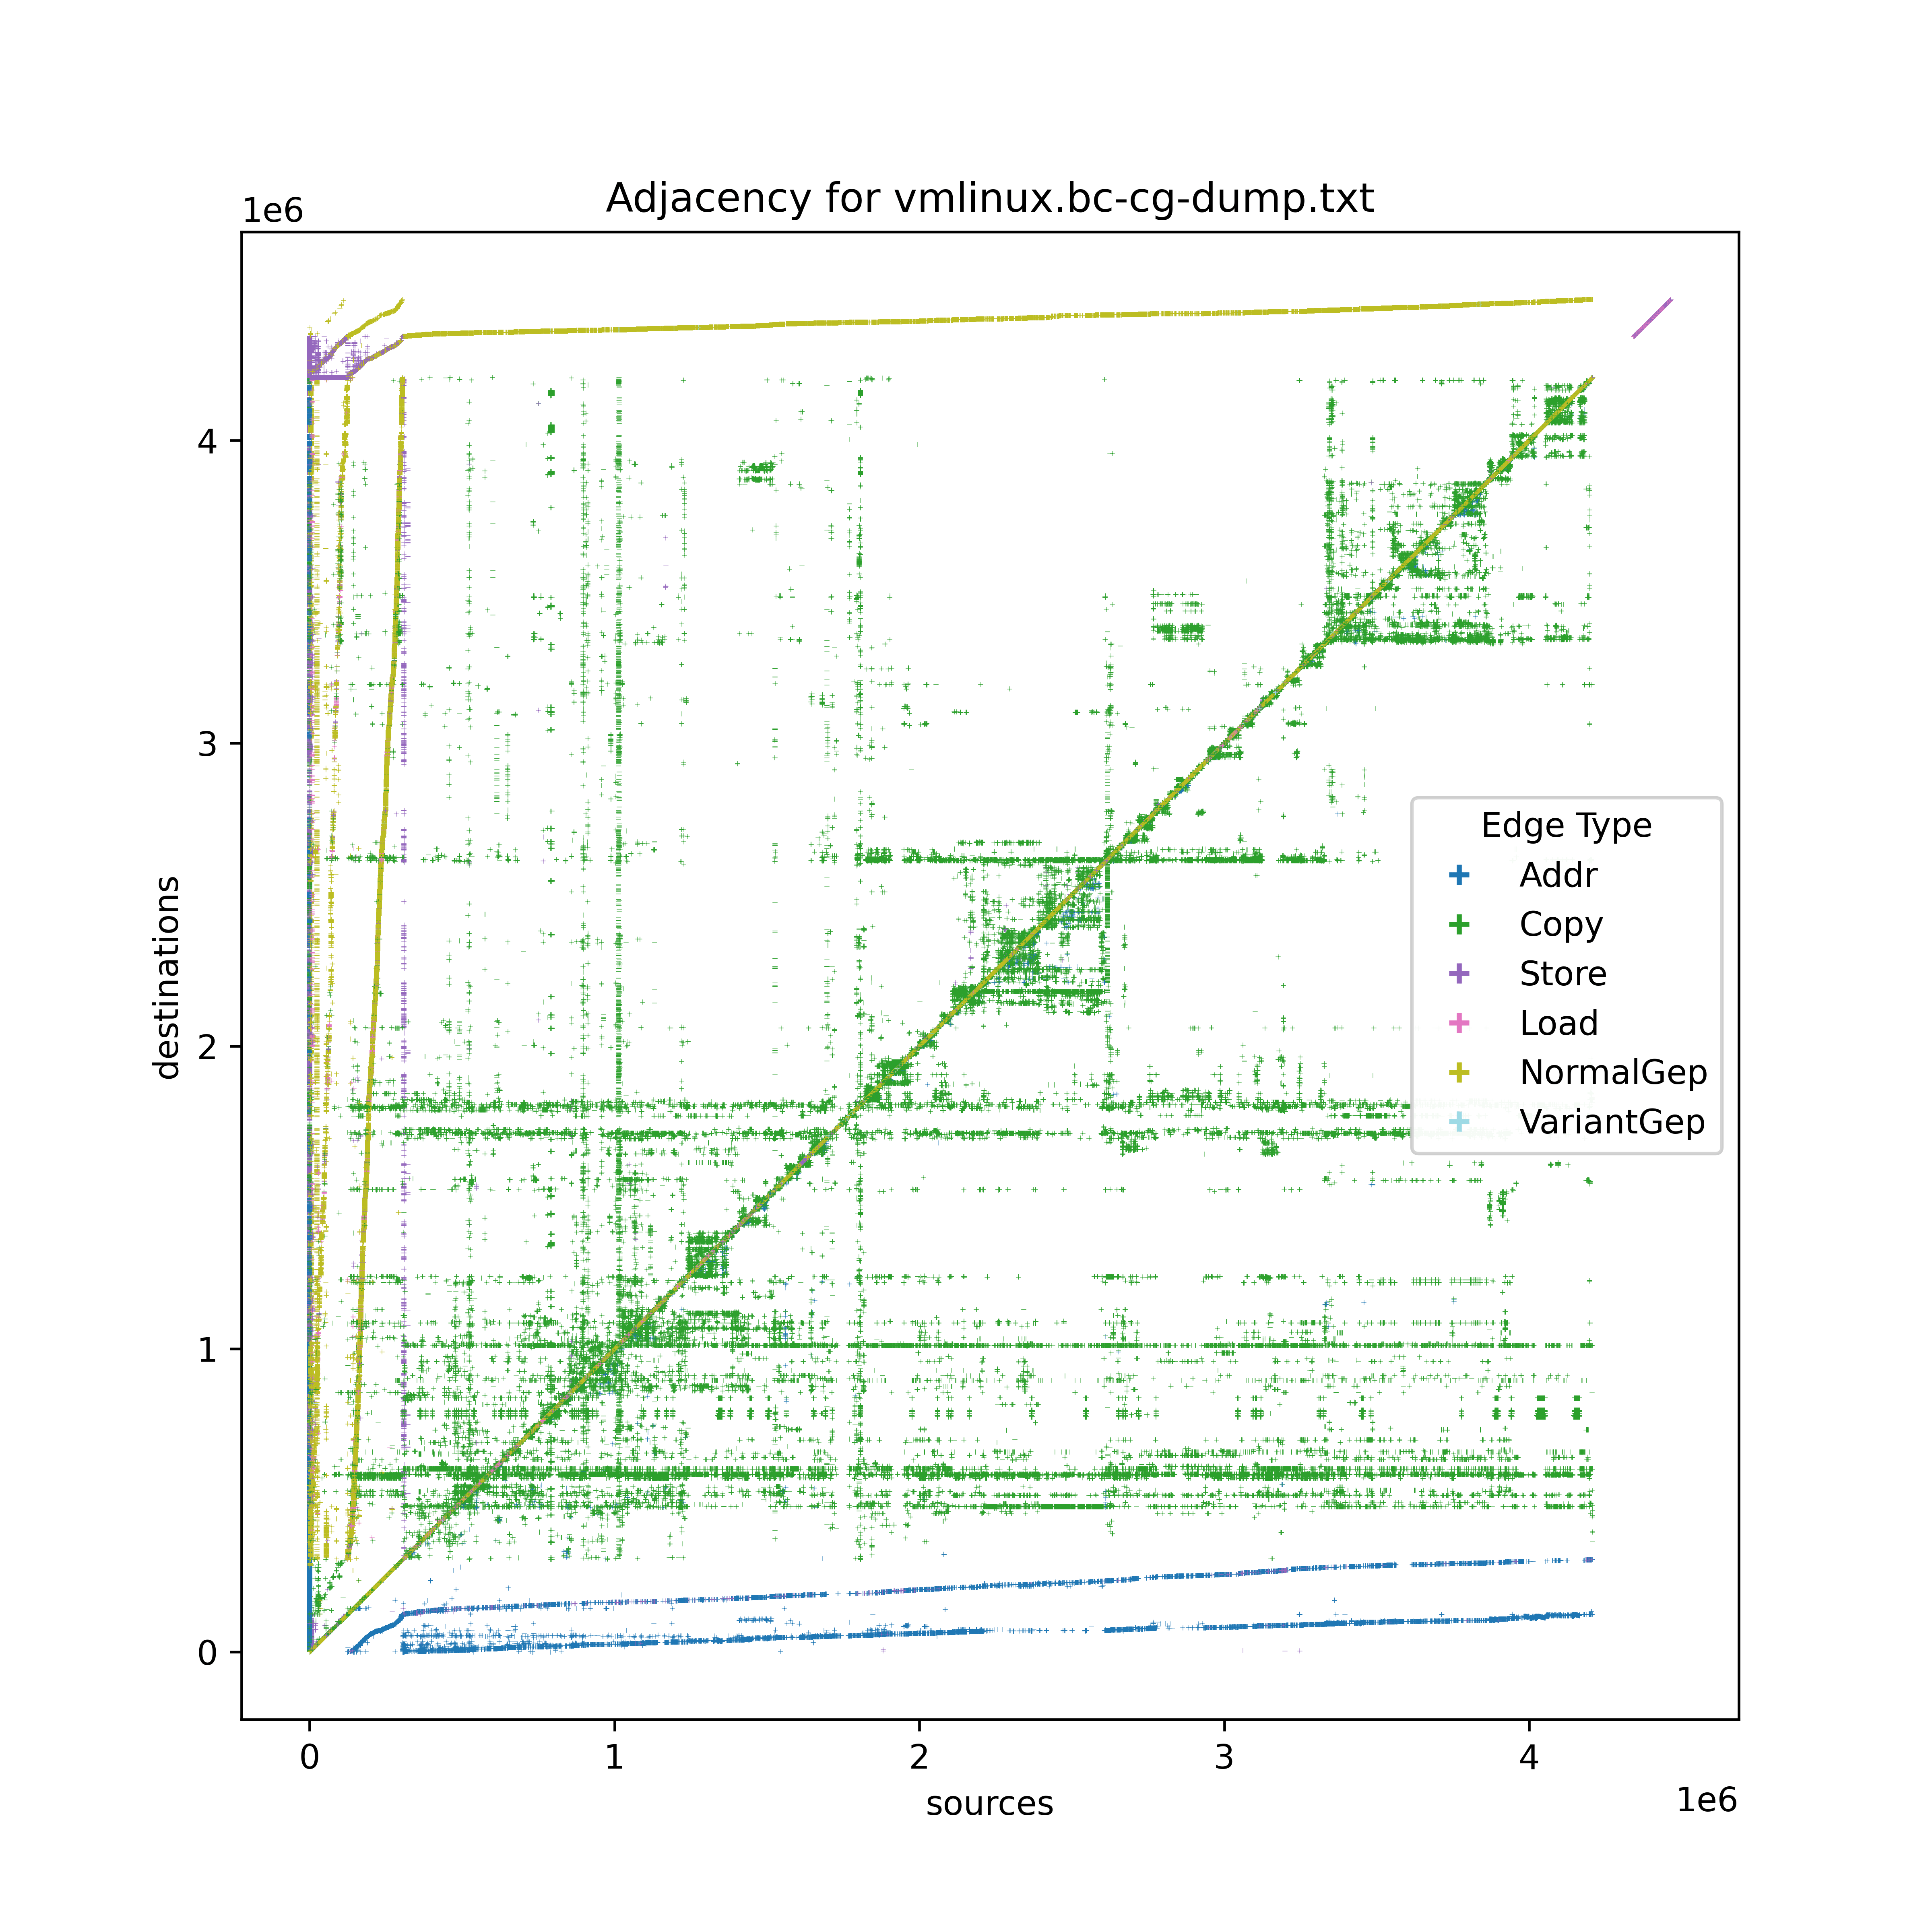
\includegraphics[width=1.\textwidth]{img/linux-consg-min.png}
    \caption{Adjacency Plot for the Constraint Graph of the Linux Kernel}
    \label{fig:linux-consg}
\end{figure}


\begin{table}[h!]
    \begin{center}
        \caption{More rows.}
        \label{tab:table1}
        \begin{tabular}{l|S|r}
            \textbf{Value 1} & \textbf{Value 2} & \textbf{Value 3} \\
            $\alpha$         & $\beta$          & $\gamma$         \\
            \hline
            1                & 1110.1           & a                \\
            2                & 10.1             & b                \\
            3                & 23.113231        & c                \\
            4                & 25.113231        & d                \\ % <-- added row here
        \end{tabular}
    \end{center}
\end{table}